\documentclass{beamer}


\usepackage{color}
\usepackage{listings}
\usepackage{courier}
\lstset{
basicstyle=\tiny\ttfamily, % Standardschrift
numbers=left, % Ort der Zeilennummern
tabsize=4, % Groesse von Tabs
}
\lstloadlanguages{C++}
%\DeclareCaptionFont{blue}{\color{blue}}
 
%\captionsetup[lstlisting]{singlelinecheck=false, labelfont={blue}, textfont={blue}}
\usepackage{caption}
\DeclareCaptionFont{white}{\color{white}}
\DeclareCaptionFormat{listing}{\colorbox{8}{\parbox{\textwidth}{\hspace{15pt}#1#2#3}}}
\captionsetup[lstlisting]{format=listing,labelfont=white,textfont=white, singlelinecheck=false, margin=0pt, font={bf,footnotesize}}

\usepackage[utf8x]{inputenc}
\usepackage{ngerman}
\usepackage{graphicx}




\title{Vernetzung, Diskretisierung der Randbedingungen}
\author{Patrick Dabbert, Stephan Hilb und Martin R\"osner}
\date{\today}

\usepackage{beamerthemesplit}


\begin{document}

\begin{frame}
	\titlepage
\end{frame}

%\begin{frame}
%	\frametitle{Inhaltsverzeichnis}
%	\tableofcontents
%\end{frame}

\section{Aufgabenstellung}

\begin{frame}
	\frametitle{Die Aufgabenstellung}
	\begin{quote}
		Entwickeln Sie Datenstrukturen, mit denen die Diskretisierung eines polygonal berandeten Gebiets $\Omega \in \mathbb{R}^{2}$ \ sowie der bei einem Randwertproblem vorgegebenen Dirichlet- oder Neumann-Daten beschrieben werden kann.
	\end{quote}
\end{frame}


\section{Beschreibung eines polygonal berandeten Gebiets}

\begin{frame}
	\frametitle{Vertex}
	\lstinputlisting{vertex.cpp}
\end{frame}

\begin{frame}
	\frametitle{Edge}
	\lstinputlisting{edge.cpp}
\end{frame}


\section{Speicherung der Dirichlet- bzw Neumann-Daten}

\begin{frame}[fragile]
	\frametitle{Das Eingabeformat}
	\lstinputlisting{Eingabedaten.cpp}

\end{frame}

\begin{frame}[fragile]
	\frametitle{Beispiel}
	\lstinputlisting{beispielgemischt.txt}
\end{frame}


\section{Bildung des Objekts ''Domain''}

\begin{frame}[fragile]
	\frametitle{Das ''Domain''-Objekt}
	\lstinputlisting{DomainObjekt.cpp}
\end{frame}



\section{Einlesen des Polygonzugs und der Randbedingungen}

\begin{frame}
	\frametitle{Einlesen der Daten}

	Definiere ein Dreieck mit den Eckpunkten $\gamma(0), \gamma(\frac 13), \gamma(\frac 23)$.
	\begin{figure}
		\caption{Anfangstriangulierung bei einer Kreiskurve}
		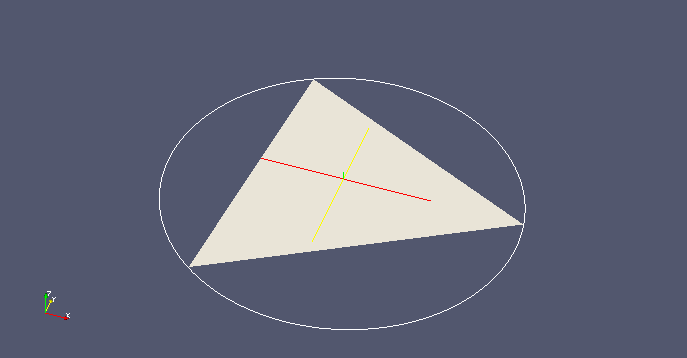
\includegraphics[width=0.8 \linewidth]{kreis0.png}
	\end{figure}
\end{frame}

\begin{frame}
	\frametitle{Vorgehen}

	\begin{enumerate}[1.]
		\item
			Halbiere jede Seite (erzeuge neuen Punkt auf der Mitte)
		\item
			Falls die Seite eine Randseite war, verschiebe den Mittelpunkt auf die Randkurve
		\item
			Erzeuge neue Dreiecke durch die eben definierten Punkte.
	\end{enumerate}
\end{frame}

\begin{frame}
	\frametitle{Kreiskurve}

	\begin{figure}
		\caption{Kreistriangulierung nach erstem Vierteln}
		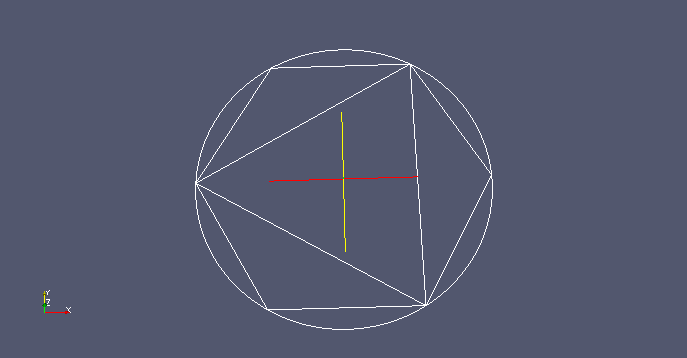
\includegraphics[width=0.8 \linewidth]{kreis1.png}
	\end{figure}
\end{frame}

\begin{frame}
	\frametitle{Kreiskurve}

	\begin{figure}
		\caption{Kreistriangulierung nach zweitem Vierteln}
		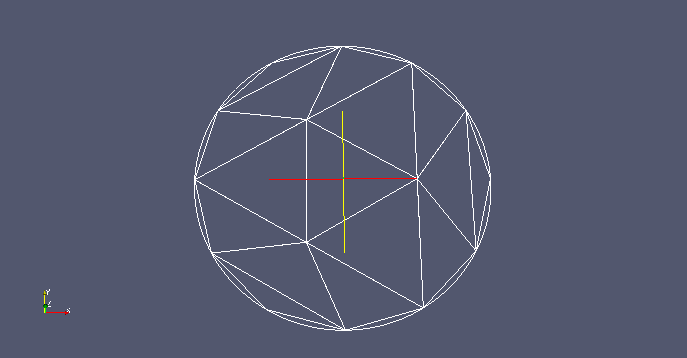
\includegraphics[width=0.8 \linewidth]{kreis2.png}
	\end{figure}
\end{frame}


\section{Alternative f\"ur Randbedingungen als Funktion}

\begin{frame}
	\begin{itemize}
		\item
			Betrachte nach jedem Verfeinerungsschritt nacheinander alle freien (nicht auf dem Rand liegende) Knoten
		\item
			FÌr jeden Knoten: verschiebe so, dass die FlÀche aller angrenzenden Dreiecke minimial wird
		\item
			Wiederhole das, solange die GesamtflÀche bei jedem Schritt um einen gewissen Prozentsatz minimiert wird.
	\end{itemize}
\end{frame}

\begin{frame}
	\frametitle{Pseudecode Beispiel}
	\lstinputlisting{minalg.cpp}
\end{frame}

\section{Generieren einer Randdiskretisierung mit Gitterweite h}

\begin{frame}
	\begin{itemize}
		\item
			Was ist die optimale oder eine gute Verschiebung?
		\item
			Welche Implementierungsmöglichkeiten gibt es?
	\end{itemize}
\end{frame}

\begin{frame}
	\frametitle{Mögliche AnsÀtze}
	\begin{itemize}
		\item
			Koordinaten der umliegenden Dreieckseckpunkte in irgendeiner Weise ''mitteln''
		\item
			Das mathematische Minimierungsproblem l\"osen
		\item
			Ein N\"aherungsverfahren verwenden (z.B. ein Gradientenverfahren)
	\end{itemize}
\end{frame}

\section{Adaptive Netzverfeinerung}

\begin{frame}
	\frametitle{Der Algorithmus}
	\begin{enumerate}[1.]
		\item
			Berechne den Gradienten des FlÀcheninhalts der umliegenden Dreiecke in AbhÀngigkeit des aktuellen Punktes
		\item
			PrÌfe, ob die FlÀche sich verkleinert, wenn der Punkt um den Gradient verschoben wird.
			Wenn ja: Verschiebe den Punkt.
			Wenn nein: Halbiere den Gradienten.
		\item
			Wiederhole 2. so lange, bis eine Verschiebung stattfindet
	\end{enumerate}
\end{frame}

\begin{frame}
	\frametitle{Code Beispiel}
	\lstinputlisting{mingradient.cpp}
\end{frame}

\begin{frame}
	\frametitle{Berechnung des Gradienten fÃŒr ein Dreieck}
	Minimiere das Dreieck $x_0,x_1,x_2$, verschiebe dabei $x_0$.

	Der Gradient ist durch die Höhe des Dreiecks durch $x_0$ in Richtung der gegenÌberliegenden Grundseite gegeben.
	Konkret:
	\[
		\big((x_0 - x_1) \times (x_0 - x_2)\big) \times (x_1 - x_2);
	\]
\end{frame}

\begin{frame}
	\frametitle{Code}
	\lstinputlisting{grad.cpp}
\end{frame}


\section{Ergebnisse}

\begin{frame}
	\frametitle{Schöne FlÀchen}
	Die meisten geschlossenen Kurven, ohne Überschneidungen liefern gute Ergebnisse.
\end{frame}

\begin{frame}
	\frametitle{Weniger schöne FlÀchen}
	Probleme bereiten
	\begin{itemize}
		\item
			offene Kurven 
		\item
			Kurven mit Überschneidungen (Viviani)
		\item
			FÀlle, in denen die Triangulierung zu stark verzerrt wird
	\end{itemize}
\end{frame}

\begin{frame}
	\frametitle{WeiterfÃŒhrende Überlegungen}	
	\begin{itemize}
		\item
			Verbesserung der Struktur des Dreiecksnetzes (möglichst gleichseitige Dreiecke)
		\item
			Bisektion statt Viertelung zur Netzverfeinerung
		\item
			Andere Strategien fÃŒr die Punktverschiebung
	\end{itemize}
\end{frame}

\begin{frame}[fragile]
	\frametitle{Ende}
	Der Quellcode und diese PrÀstentation sind zu finden auf
	\begin{verbatim}
		https://github.com/stev47/cp/tree/master/projekt1
	\end{verbatim}
\end{frame}




\end{document}
